\documentclass{beamer}

\usepackage[utf8x]{inputenc}
\usepackage[T1]{fontenc}
\usepackage[ngerman]{babel}
\usepackage{amsmath,amsfonts,amssymb}
\usepackage{lmodern}
\usepackage{marvosym}

\usetheme{Berlin}

\begin{document}
    \author{Pascal Kn"uppel, Dirk Evers, Jan-Bernd Vosteen}
    \title{Design f"ur Analphabeten}
    \date{22.01.2013}
    
    \frame{\titlepage}
    
    \frame{\frametitle{Inhaltsverzeichnis}\tableofcontents}

	\section{Einleitung}



In unserem derzeitigen Zeitalter der Kommunikation über technische Medien kommen wir zu keinem Tag drum herum einen Text vor uns zu sehen. Der Text an sich ist zu einer allgemeinen abstrakten Kommunikationsschnittstelle geworden, der wir Menschen uns bedienen und mit der wir uns exakt untereinander und sogar mit Maschinen verständigen können. Text dient dazu, um Informationen zu speichern/archivieren, sich selbst nach außen hin zu präsentieren, Geschichten zu erzählen und vieles mehr.\\


Und doch gibt es viele Menschen, die in Deutschland und auf dem Rest der Welt, weder lesen noch schreiben können. In Deutschland alleine gibt es ca. 7,5 Millionen Menschen, das sind etwa 6\% der Bevölkerung, denen diese wichtige Fähigkeit versagt ist. Auf der ganzen Welt hingegen gibt es ungefähr 775 Millionen Menschen, die das Lesen und Schreiben nicht beherrschen. \\


 Wie also sollen diese Menschen in der heutigen Welt zurecht kommen? Befindet sich einer aus dieser Gruppe bspw. in einem Restaurant, wie soll es ihm möglich sein, etwas von der Karte zu bestellen? Wie soll so eine Person herausfinden, welchen Bus sie nehmen muss, um wieder nach Hause zu kommen? Wie soll sie sich bewerben, um einen Job zu kriegen, wenn sie ihren eigenen Lebenslauf nicht schreiben kann? Diesen und vielen weiteren Problemen sind diese Menschen Tag für Tag ausgesetzt. Es ist ein ständiger Kampf für sie in der Welt, die von Texten beherrscht wird. Deshalb wollen wir in dieser Ausarbeitung darauf eingehen, wie man Designs so auslegen kann, dass selbst Leute, die des Lesens nicht mächtig sind, mit diesen Objekten zurecht kommen.\\
 Wir werden im ersten Abschnitt darauf eingehen, mit welchen Begriffen diese Menschen beschrieben werden, wie wir sie klassifizieren, also welche Unterschiede es zwischen Menschen gibt, die nicht Lesen und Schreiben können. Dann gehen wir weiter zu den Gründen, wieso diese Menschen das Lesen und Schreiben nicht gelernt haben, oder es nicht lernen konnten, wozu wir dann ebenfalls den Erfahrungsbericht einer solchen Person vorstellen, die über eine sehr lange Zeit ein solches Leben geführt hat.\\
 Im Anschluss werden wir dann verschiedene Konzepte vorstellen, die es zu berücksichtigen gilt, wenn Designs entwickelt werden sollen, die auch den Anforderungen dieser Menschen entsprechen.


\subsection{Definition}



Die eben erwähnten Menschen, die nicht lesen und nicht schreiben können, werden im Volksmund "`Analphabeten"' genannt. Es stimmt jedoch nicht, dass diese Leute überhaupt nicht lesen und schreiben können. Der Großteil der Analphabeten kann in einem begrenzten Maße lesen und ist dazu in der Lage, einige Wörter zu schreiben.\\

Somit wäre eine gängige Definition für Analphabeten:\\
\begin{itemize}
	\item \textbf{\textit{Menschen, die das Lesen und Schreiben nicht, bis nur teilweise beherrschen.}}
\end{itemize}



\subsection{Arten des Analphabetismus}

Der Analphabetismus wird von Fachleuten, wie auf der Seite vom "`Bundesverband Alphabetisierung und Grundbildung e.V."'
\footnoteSource {Bundesverband Alphabetisierung und Grundbildung e.V.}
				{Analphabetismus}
				{02.06.2013}
				{http://www.alphabetisierung.de/infos/analphabetismus.html}, 
in verschiedene Kategorien eingeteilt. Da die Menschen in der Regel aus verschiedenen Gründen nicht richtig lesen und schreiben können, scheint eine solche Unterteilung auch durchaus sinnvoll:

\begin{itemize}
	\item primärer Analphabetismus
				\begin{itemize}
					  \item Ein primärer Analphabet ist jemand, der das Lesen und Schreiben niemals gelernt hat.
				\end{itemize}
	\item sekundärer Analphabetismus
				\begin{itemize}
					  \item Ein sekundärer Analphabet ist jemand, der das Lesen und Schreiben ursprünglich mal erlernt hat, es aber wieder verlernte, da er diese Fähigkeit nie einzusetzen brauchte.
				\end{itemize}
	\item Semianalphabetismus
				\begin{itemize}
					  \item Ein Semianalphabet ist jemand, der des Lesens, aber nicht des Schreibens mächtig ist.
				\end{itemize}
	\item funktionaler Analphabetismus
				\begin{itemize}
					  \item Ein funktionaler Analphabet ist jemand, der einzelne Worte lesen und schreiben kann, dem es aber nicht möglich ist, längere Texte vollständig zu erfassen und zu verstehen.\\
						(Dieser Typ des Analphabetismus macht den größten Teil der Analphabeten aus und ist auch in Deutschland besonders stark vertreten.)
				\end{itemize}
\end{itemize}
	
	\section{Gründe für Analphabetismus}

	\subsection{Gründe für Analphabetismus}
		
\frame{\frametitle{Gründe des Analphabetismus}
	
	
		\begin{enumerate}
		
			\item Mangelnde Bildung \pause
			
			
			\item Legasthenie
			\begin{itemize}
				\item Eine Störung der auditiven und visuellen Wahrnehmungsverarbeitung.
			\end{itemize}\pause
			
			
			\item Dyslexie
			\begin{itemize}
				\item Wörter und/oder Texte, werden kognitiv nicht richtig verstanden.
			\end{itemize}\pause
			
			
			\item Agrafie
			\begin{itemize}
				\item Wörter können nicht geschrieben werden, trotz normalen Intellekts und guter Handmotorik
			\end{itemize}
		\end{enumerate}
	
	}
	
		

\frame{\frametitle{Mangelnde Bildung}

	Hauptursachen sind nach Untersuchungen häufig folgende:
 	\begin{itemize}
		\item Kinder werden ausgelacht beim Vorlesen\pause
		\item von den Eltern nicht unterstützt\\
			Sätze wie "`du bist sowieso zu dumm"' demotivieren die Kinder\pause
		\item Lehrer werden nicht aufgeklärt und bestrafen die Kinder bei schlechter Leistung\pause
		\item demotivierte Kinder mogeln sich im Folgenden durch und wollen ihre Schwäche geheim halten
	\end{itemize}

 }
		
\frame{\frametitle{Legasthenie}
	\begin{itemize}
 		\item Eine Störung der auditiven und visuellen Wahrnehmungsverarbeitung, die zu einer Lese- und Rechtschreibschwäche führt, trotz normal entwickelter Intelligenz. \pause
 		\item erblich bedingt \pause
 		\item taucht häufig gemeinsam mit AD(H)S auf\pause
 		\item umstritten ob heilbar oder nicht
 	\end{itemize}
 }

\frame{\frametitle{Legasthenie}

 	\begin{figure}[t]
	\centering
		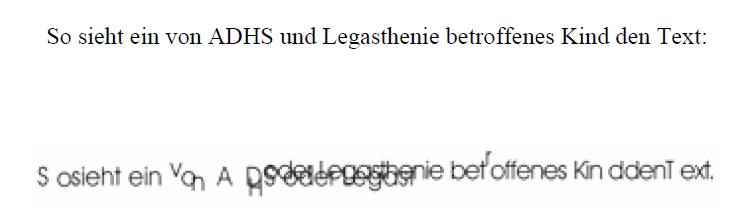
\includegraphics[width=1.0\textwidth]{Slides/Gruende/Daten/legastheneWahrnehmung.PNG}
	\end{figure}
 }

	
	\section{Analphabeten im Alltag}

	\subsection{Probleme der Analphabeten}
	
	

\frame{\frametitle{Analphabeten im Alltag}

 	
 }

	\section{Design f"ur Analphabeten}
Da das Design in den meisten Anwendungen von Texten abh"angig ist, sind Analphabeten mit diesen Anwendungen "uberfordert, da sie keine M"oglichkeit haben, zu verstehen, was Ihnen vorliegt. \\
Um also eine technische Anwendung so zu gestalten, dass auch Analphabeten sie verstehen, sollte man zwei verschiedene Ans"atze betrachten.

Das Design ist f"ur ...
\begin{enumerate}
	\item prim"are/sekund"are Analphabeten gedacht und wird lediglich "uber Bild- und Tonmedien gestatltet.
	\item funktionale Analphabeten gedacht, was die Verwendung von Text in geringem und einfach verst"andlichem Ma"se noch zul"asst. Jedoch sollten auch hier Bild und Tonmedien im Vordergrund stehen.
\end{enumerate}

\subsection{Designentwicklung}\label{sec:designEval}
Um die Benutzerfreundlichkeit f"ur Analphabeten zu "uberpr"ufen m"ussen, Analphabeten als Testgruppen herangezogen werden. Die Testgruppen zum Analphabetismus sind aufgrund ihrer Verschwiegenheit schwer zu finden. So empfiehlt es sich mit  Hilfsorganisationen wie \glqq Alphabund\grqq{}  zusammenzuarbeiten. Hier k"onnen auch oft bereits get"atigte Studien angefordert werden. Dabei stammen die Studien zu funktionalen Analphabeten vorwiegend aus den Industriestaaten und die Studien zu prim"aren und sekund"aren Analphabeten meist aus Entwicklungsl"andern wie Indien und den Philippinen,  wie in der Studie aus Kapitel \ref{sec:beisp3}. Bei Testgruppen aus anderen L"andern m"ussen auch andere kulturelle Faktoren beachtet werden wie im Vortrag \glqq Design und Kultur\grqq{}.  \footnoteSource{\label{W.M.Gribbons01}William M. Gribbons}
					{Universal Accesibility and Low-Literacy Populations, Implications for Human-Computer, Interactions Design and Research Methods}
					{2012}
					{The Human-Computer Interaction Handbook: Fundamentals, Evolving Technologies and Emerging Applications}
\footnoteSource{\label{MedhiSaraToyama01}Indrani Medhi, Aman Sagar, and Kentaro Toyama}
					{Text-Free User Interfaces for Illiterate and Semi Literate Users}
					{2006}{}
Bei der Arbeit mit den Analphabeten innerhalb der Studien, m"ussen die "ublichen Schriftst"ucke wie Aufgabenliste oder Frageb"ogen ersetzt werden. Entweder m"ussen sie durch Bild- oder Sprachaufnahmen ersetzt werden, oder der Proband wird pers"onlich begleitet.
Da Analphabeten ge"ubt sind im Auswendiglernen von W"ortern und T"atigkeiten m"ussen die Probanden h"aufiger als "ublich ausgetauscht werden, um zu gew"ahrleisten, dass die Anwendung tats"achlich intuitiv ist.$^{\ref{W.M.Gribbons01}}$\\
\newpage

\subsection{ Designfolgerungen}\label{sec:designClue}
Wie bereits erw"ahnt gibt es zwei grundlegende Varianten zum Design f"ur Analphabeten.
\begin{itemize}
\item Das Verwenden von Bildern und/oder Tonaufnahmen statt Texten f"ur prim"are und sekund"are Analphabeten.
\item Das Vereinfachen und Unterst"utzen von Texten f"ur eine breitere Benutzergruppe.
\end{itemize}
Die Variante f"ur prim"aren und sekund"aren Analphabetismus unterscheidet sich haupts"achlich im Vermeiden von Texten von der Variante f"ur funktionale Analphabeten. Darum wird im Folgenden haupts"achlich auf die Variante f"ur funktionale Analphabeten eingegangen.

Im Kapitel \glqq Universal Accesibility and Low-Literacy Populations, Implications for Human-Computer, Interactions Design and Research Methods\grqq{}$^{\ref{W.M.Gribbons01}}$ aus dem Buch \glqq The Human-Computer Interaction Handbook: Fundamentals, Evolving Technologies and Emerging Applications\grqq{} beschreibt W.M.Gribbons die Folgerungen f"ur das Design der Analphabeten in vier Kategorien:\\

\begin{itemize}
\item Lesen:              "Anderungen die das Lesen der einzelnen W"orter vereinfachen oder auch ersetzen.
\item Merken:            "Anderungen die das Merken vereinfachen und somit die Konzentration erh"ohen.
\item Metakognition: "Anderungen die zum Schlussfolgern und verstehen des Inhalts n"otig sind.
\item Suche und Navigation : "Anderungen die die Suche in der Anwendung und das Suchen von Informationen erleichtern.
\end{itemize}

\subsubsection{Lesen}\label{sec:designClueReading}

F"ur prim"are und sekund"are Analphabeten, muss der Textinhalt vollst"andig durch andere Medien ersetzt werden. Neben einfachen Signalen wie Piept"onen k"onnen auch Tonaufnahmen oder Screenreader verwendet werden, wie im Vortrag zum Thema  \glqq Design f"ur Menschen mit Sehsch"adigung\grqq{} vorgestellt.
Ebenfalls k"onnen Illustrationen verwendet werden, welche "uber ihren Bildinhalt die selben Informationen vermitteln.
Da Illustrationen aber wesentlich komplexer als Texte sind, m"ussen sie m"oglichst Aussagekr"aftig und leicht interpretierbar sein. Dabei gilt es, wie auch im Vortrag \glqq Globalisierung, Lokalisierung\grqq{} die kulturellen Unterschiede strikt zu beachten.\\
F"ur funktionale Analphabeten muss der Text nicht zwingend ersetzt werden, doch ist es dann wichtig, den Text einfacher und verst"andlicher zu gestalten. Damit wird der Text verst"andlicher f"ur funktionale Analphabeten und sollte durch die bisher genannten alternativen Medien erg"anzt werden. Um das Lesen des Textes zu vereinfachen, sollten die Informationen auf das wesentliche reduziert und in sinnvolle Gruppen gegliedert werden. Auch hilft es den Text in einfacherer Sprache zu schreiben. Denn je nach verwendetem Wortschatz ist der Text einfacher, oder auch schwerer zu verstehen. Ein Beispiel dazu ist in Abbildung \ref{fig:GoerFive} zu finden. Hier erkl"art Randall Munroe mit Hilfe der 1000 bekanntesten englischen W"orter den Aufbau der Saturn V Rakete.
\footnoteSource{\label{up_goer_five_01}Jason Major}
				{This is Awesome: U.S. Space Team’s “Up Goer Five”}
				{5.6.2013}
				{http://www.universetoday.com/98411/this-is-awesome-u-s-space-teams-up-goer-five/}

\begin{figure}[h]
	\centering
		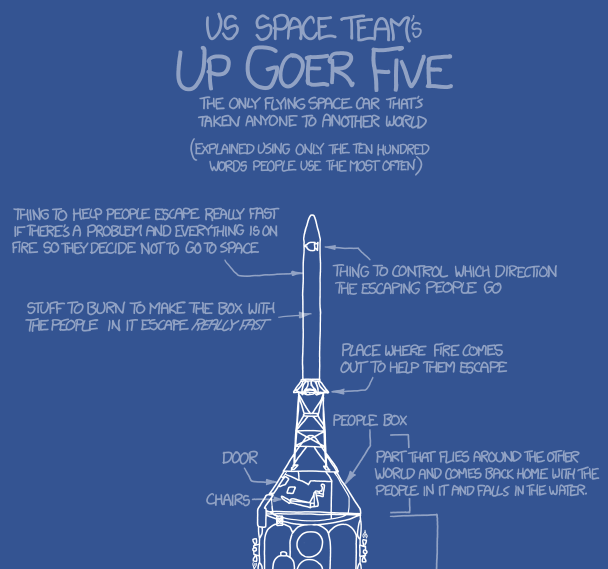
\includegraphics[width=0.50\textwidth]{Daten/up_goer_five_part.png}
	\caption{Up Goer Five: Einfache Sprache aber schwierige Schrift $^{\ref{up_goer_five_01}}$}
	\label{fig:GoerFive}
\end{figure}
 Durch die einfache Sprache f"allt es dem Leser einfacher den Inhalt des Textes zu verstehen. Doch wird eine ung"unstige Schriftart verwendet, welche f"ur unge"ubte Leser schwerer zu lesen ist, hilft auch ein einfach formulierter Text nicht mehr, da auch die Schriftart einen Einfluss auf den Schwierigkeitsgrad eines Textes hat.
Um den Inhalt eines Textes zu kategorisieren, f"uhrten Croft und Peterson 2002 und Darrell West 2003 Arbeiten durch, in denen sie Schriftst"ucke mehreren Wortsch"atzen von unterschiedlicher Schwierigkeit zuordneten.
Demnach liegen etwa 70\% der staatlichen Webseiten auf einem Level von 12 und Asthma bezogene Webseiten auf einem Level von 10.
Dabei beherrscht die H"alfte der amerikanischen Bev"olkerung h"ochstens Level 8. Ein funktionaler Analphabet liegt noch weit darunter.
Ein Schriftst"uck von Level 8 kann somit von allen Amerikanern verstanden werden, ein Schriftst"uck mit deutlich niedrigerem Level jedoch auch von anderen Gruppen bis hin zu den funktionalen Analphabeten.$^{\ref{W.M.Gribbons01}}$\\

\subsubsection{Merken}
Das Merken hat nur indirekte Auswirkungen auf das Leseverhalten. Einerseits f"uhren einige mentale Behinderungen die sich auf das Merken auswirken zum Analphabetismus wie es schon im Vortrag \glqq Design f"ur Menschen mit Lernschwierigkeiten\grqq{} erw"ahnt wurde. Andererseits kann eine Person nur eine bestimmte Menge an Konzentration aufwenden. Ist Diese bereits f"ur das Merken verbraucht, fehlt die Konzentration beim Lesen, oder es werden Informationen vergessen und Passagen m"ussen erneut gelesen werden. Die F"ahigkeit zu Merken kann unterst"utzt werden, indem die Informationen aufs wesentliche Reduziert werden, oder in sinnvolle Gruppen gegliedert werden. Am wichtigsten ist jedoch, dass unn"otige Ablenkungen vermieden werden.
Die offensichtlichen Ablenkungen sind blinkende Werbebanner, Lauftext oder aber auch zu viele Nebenaufgaben. Denn mit vielen Aufgaben m"ussen nicht nur mehr Informationen verarbeitet werden, sondern auch der Informationswert f"ur die einzelnen Aufgaben ermittelt werden. F"ur den Inhalt selber ist es wichtig, dass Widerspr"uche m"oglichst vermieden werden. Denn Widerspr"uche zwingen den Benutzer, die Informationen erneut durchzugehen und zu bewerten und die Kapitel erneut zu lesen.

\subsubsection{Metakognition}

Die Metakognition beschreibt das Verarbeiten und Kombinieren der gesammelten Informationen und "uberschneidet sich in einigen Punkten mit den anderen Kategorien. Um die Metakognition zu verbessern, sollte die Anwendung m"oglichst einheitlich gehalten werden, damit der Benutzer m"oglichst nicht mit vielen verschiedenen Interfaces auseinandersetzen muss. Um das Zielsetzen zu erleichtern, kann die Anwendung bereits das Ziel vorgeben. So sieht der Benutzer z.B. das er sich erst anmelden muss. Auch kann eine "Ubersicht der Ziele mit zuk"unftigen und bereits abgeschlossenen Zielen in Form einer Checkliste sinnvoll sein. Ein Beispiel f"ur solche Checklisten ist die Installationssoftware vom Microsoft-Server 2007
\footnoteSource{\label{ mc_serv_01}Microsoft}
						{Microsoft-Server 2007 Installation}
						{Stand : 14.2.2013}
						{http://i.technet.microsoft.com/dynimg/IC22550.gif} 
aus der Abbildung \ref{fig:InstallBsp}. Hier Rot markiert sind die einzelnen Installationsschritte w"ahrend der gesamten Installation einsehbar.\\
\begin{figure}[h]
	\centering
		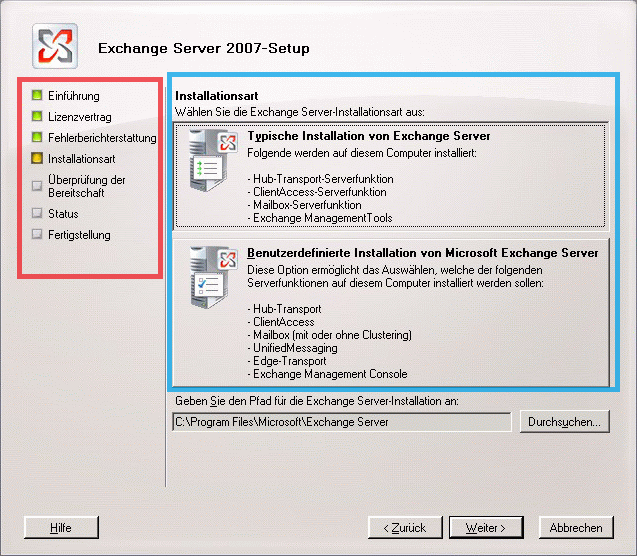
\includegraphics[width=1.00\textwidth]{Daten/ServerBeispiel.png}
	\caption{Interface mit Checkliste und Wahlm"oglichkeiten $^{\ref{ mc_serv_01}}$}
	\label{fig:InstallBsp}
\end{figure}
Auch ein Men"u oder eine einfache Auswahl kann sehr fordernd f"ur Analphabeten sein. Diese Wahlm"oglichkeiten sollten m"oglichst eindeutig, dabei aber auch nicht zu kompliziert beschrieben sein. Da diese Anwendungen zumeist jedoch nicht auf diesem niedrigem Level gehalten sind, verwenden Analphabeten h"aufig
einfach die erste M"oglichkeit. In manchen F"allen kann dieses Verhalten ausgenutzt werden, indem man die Auswahl f"ur Analphabeten optimiert. So kann im Beispiel aus der Abbildung \ref{fig:InstallBsp} mit Blau markiert, die Auswahl "uber den Installationsumfang getroffen werden. Die erste Variante bietet hier eine vordefinierte Auswahl und ist somit Ideal f"ur einen Analphabeten.$^{\ref{W.M.Gribbons01}}$\\


\subsubsection{Navigation und Suche}
\begin{figure}[h]
	\centering
		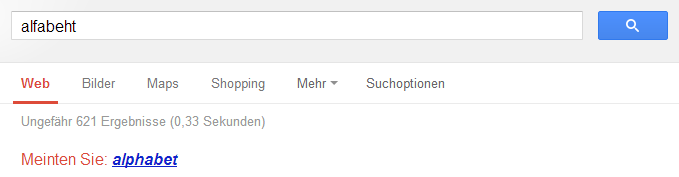
\includegraphics[width=0.80\textwidth]{Daten/rechtschreibung.png}
	\caption{Fehlerkorrektur der Suche bei Google $^{\ref{google01}}$}
	\label{fig:GoogleSearch}
\end{figure}

"Ubersicht ist f"ur jeden Benutzer sinnvoll. Jedoch ist es schwer die Balance zwischen vielen Wahlm"oglichkeiten und der Tiefe der Wahlm"oglichkeiten zu finden. Gerade zum Unterscheiden der M"oglichkeiten sollte klar sein, wohin welche Auswahl f"uhrt, damit sich
 die Suchwege m"oglichst verk"urzen. Eine weitere Variante um den Suchweg zu verk"urzen, ist den Verlauf anzuzeigen, damit der Benutzer zur"uck verfolgen kann, was er bereits bearbeitet hat. Ebenso sollten die wichtigsten oder auch h"aufigsten Inhalte wie Suche, Anmelden und Hilfe m"oglichst ohne Suchen zug"anglich sein.\\
Die Suche stellt f"ur Analphabeten eine besondere Herausforderung dar. Die "ubliche Suche ben"otigt eine genaue Eingabe des zu suchenden Wortes. Da funktionale Analphabeten die W"orter h"aufig falsch schreiben, kommen sie gew"ohnlich nicht an das gew"unschte Ziel. Darum sollte die Suche die Eingabe erst interpretieren und gegebenenfalls Alternativen anbieten.
Als g"angigstes Beispiel hierf"ur dient die Suchmaschiene Google$^{\ref{fig:GoogleSearch}}$, welche z.B. \glqq alfabeht\grqq{}  als Korrektur f"ur \glqq alphabet\grqq{}  angibt.
\footnoteSource{\label{google01}Google Inc.}
						{Google Suchmaschiene}
						{Stand : 5.6.2013}
						{www.google.de}

\subsection{Beispiele: Design f"ur Analphabeten}
In diesem Kapitel folgen drei Beispiele f"ur Anwendungen, die f"ur Analphabeten geeignet sind und die die in \ref{sec:designClue} genannten Kriterien verdeutlichen sollen. Dabei wurden m"oglichst verschiedene Anwendungen gew"ahlt, um zu zeigen auf welch unterschiedliche Arten Anwendungen f"ur Analphabeten funktionieren k"onnen..$^{\ref{W.M.Gribbons01}}$\\


\subsubsection{ integrierte Software: ReadSpeaker}

Dieses Beispiel ist eine integrierte Software, welche beliebigen Text der Webseite Bundesverband Alphabetisierung
\footnoteSource{\label{alphaBund01}Bundesverband Alphabetisierung}
						{Bundesverband Alphabetisierung Website}
						{Stand : 14.2.2013}
						{http://www.alphabetisierung.de/}
vorlesen kann.
Dabei markiert der Benutzer den zu "ubersetzenden Text, worauf unten rechts eine Schaltfl"ache \glqq Vorlesen\grqq{} wie in Abbildung  \ref{fig:DesignBeispiel1} erscheint. Mit dieser kann nun die Wiedergabe gestartet werden, worauf wieder eine weitere Schaltfl"ache erscheint, mit der unter anderem die Wiedergabe gestoppt oder pausiert werden kann.\\
Somit wird der Umfang der Website f"ur funktionale Analphabeten weit gesteigert und sogar prim"are Analphabeten d"urften sp"atestens nach einer kleinen Einweisung den Umfang nutzen k"onnen. Auch ist nur die Maus als Eingabeger"at n"otig. So kann eine beliebige Seite mit beliebigem Inhalt, vom Anbieter, leicht f"ur den Analphabeten zug"anglich gemacht werden. Dabei kann bis auf in Bildern vorkommender Text, jeder Text ohne teure Tonaufnahmen "ubersetzt werden, wie in \ref{sec:designClueReading}. Dabei geht aber die "Ubersichtlichkeit verloren, da es f"ur den Benutzer dauert, den Text zu markieren und anzuh"oren. Au"serdem ist der Wortschatz nicht unbedingt f"ur Analphabeten geeignet und durch den "Ubersetzer schwer zu verstehen.
\begin{figure}[h]
	\centering
		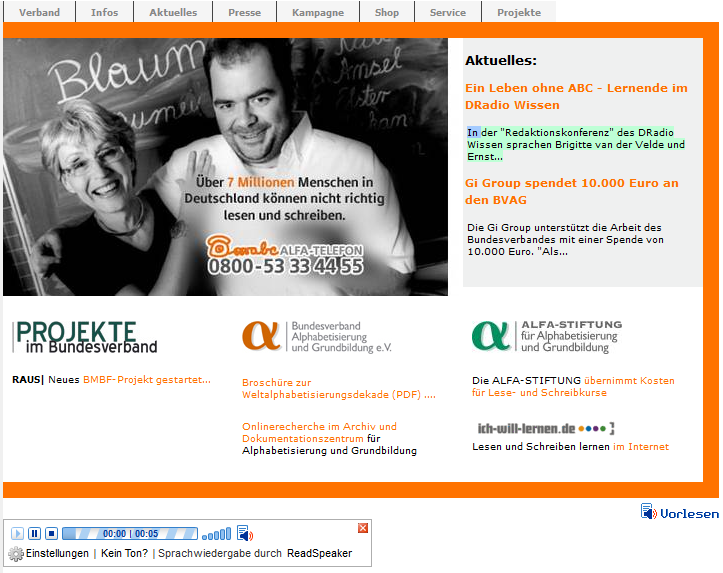
\includegraphics[width=0.80\textwidth]{Daten/DesignBeispiel1.png}
	\caption{Design Beispiel vom Bundesverband Alphabetisierung $^{\ref{alphaBund01}}$}
	\label{fig:DesignBeispiel1}
\end{figure}

\newpage

\subsubsection{Reines Text-Design : Invisque}
Dieses Beispiel zeigt eine Anwendung, welche sich nur f"ur funktionale Analphabeten eignet: Die Suchmaschine Invisque (INteractive VIsual Search and QUery Environment)
\footnoteSource{\label{Invisque01}Invisque - INteractive VIsual Search and QUery Environment}
						{Stand: 5.6.2013}
						{http://www.invisque.com/index.html}{}
.\\
Diese Suchmaschine ist nicht in erster Linie nur f"ur Analphabeten entwickelt worden, wurde aber laut Angaben der Entwickler so weiterentwickelt, dass sie auch f"ur funktionale Analphabeten geeignet ist. Um dieses Ziel zu erreichen, haben die Entwickler versucht, einigen Problemen der funktionalen Analphabeten entgegen zu wirken, wie z.B., dass es diesen Menschen schwer f"allt sich auf den Text zu konzentrieren, wenn sehr viel ablenkender weiterer Text auf der Seite verteilt wird, oder wenn PopUps auftauchen, oder allgemein blinkende Werbung an den R"andern die Aufmerksamkeit auf sich zieht. All dies blendet Invisque erfolgreich mit einer Blanko-Oberfl"ache aus. Invisque verwendet einen wenig irritierenden wei"sen Hintergrund. In den Ecken befinden sich kleine Felder, aus denen weitere Informationen und Navigationsunterst"utzung gew"ahlt werden k"onnen, wie auf Abb.\ref{fig:Invisque} zu sehen ist.

\begin{figure}[h]
	\centering
		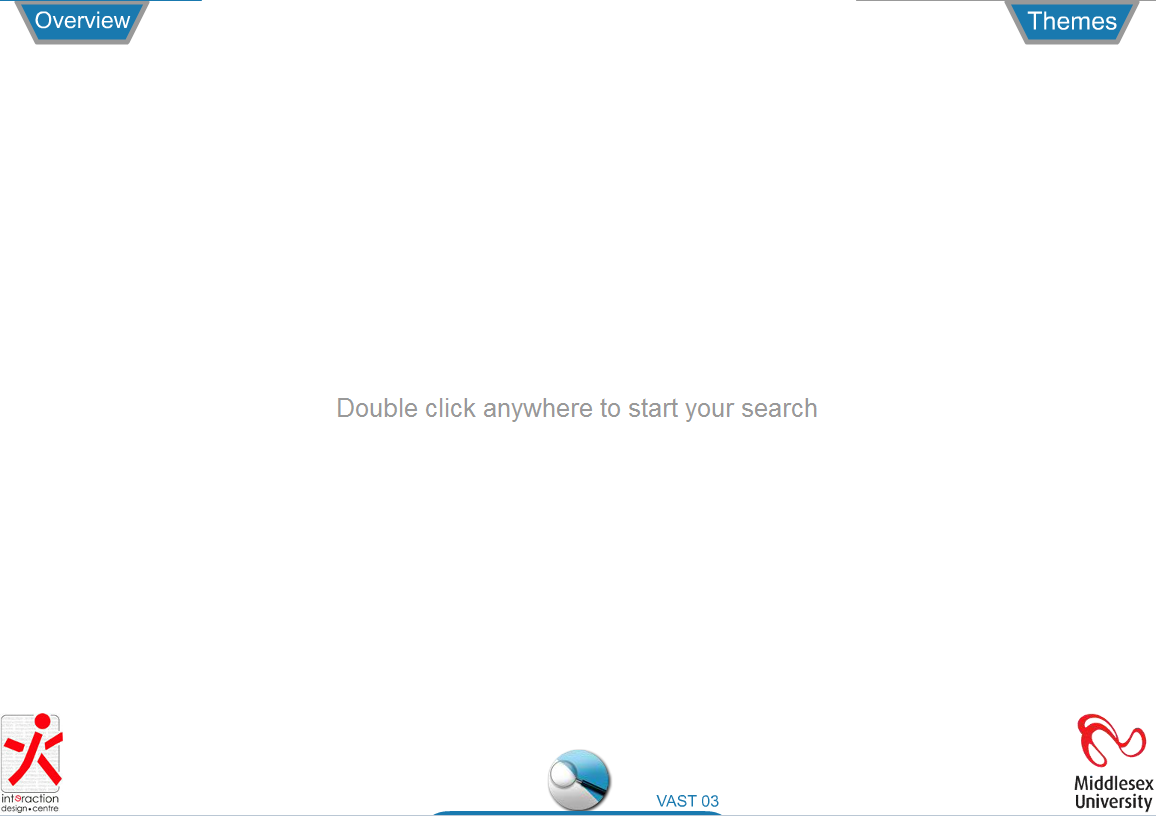
\includegraphics[width=0.80\textwidth]{Daten/Inisque.PNG}
	\caption{Invisque Oberfl"ache}
	\label{fig:Invisque}
\end{figure}

Um einen guten "Uberblick "uber diese Suchmaschine zu bekommen, ist es zu empfehlen sie selbst auszuprobieren und verschiedene Schl"usselw"orter einzugeben.

\newpage
\subsubsection{Textlose Anwendung}\label{sec:beisp3}
In diesem Beispiel geht es um zwei Anwendungen, die zur Studie \glqq Text-Free User Interfaces for Illiterate and Semi Literate Users\grqq{}
\footnoteSource{\label{MedhiSagarKentaro01}Indrani Medhi, Aman Sagar, and Kentaro Toyama}
					{Text-Free User Interfaces for Illiterate and Semi Literate Users}
					{2006}
					{}
 von Indrani Medhi, Aman Saga und Kentaro Toyama geschrieben wurden.\\
Ziel war es Anwendungen zu schreiben, welche einer indischen Slumbev"olkerung eine erleichterte Jobsuche und Orientierungshilfe mit den Standorten der Jobs bieten sollte. Die Inspiration zu diesem Projekt r"uhrte daher, dass die Menschen dort aufgrund ihrer Leseschw"ache und weil sie ihre Wohngegenden selten verlassen, nicht "uber andere Jobangebote informiert sind, was dazu f"uhrt, dass sie h"aufig f"ur ein viel zu niedriges Einkommen arbeiten, obwohl es in der erreichbaren Umgebung meist viele bessere Angebote gibt. Da die Bev"olkerung vorwiegend aus prim"aren Analphabeten besteht, entschieden sich die Entwickler, wie in  \ref{sec:designEval} beschrieben, die Anwendung nur aus Bildern zu gestalten. Aber gerade bei diesen Bildern war es wichtig, den kulturellen Hintergrund der Bev"olkerung zu beachten. Zum Beispiel hatte kaum ein Bewohner Erfahrung mit digitaler Technik.\\
Besonders wurde die Interpretationen der Bilder hervorgehoben. Bilder welche 2ur die Entwickler leicht zu deuten waren, waren f"ur die Menschen dort missverst"andlich. So mussten f"ur Bilder wie Absp"ulen und Kochen noch zus"atzlich Feuer und Wasser hinzugef"ugt werden, wie man in Abbildung \ref{fig:picfail} sehen kann. (Zur Veranschaulichung haben wir das Bild um die Illustrationen ohne Feuer und Wasser erweitert.) Hier wurden die linken Darstellungen eher als Geschirr angesehen, statt den gewollten Aktionen Absp"ulen und Kochen. Somit wurden sie durch die rechten Darstellungen ersetzt.\\\\

\begin{figure}[h]
	\centering
		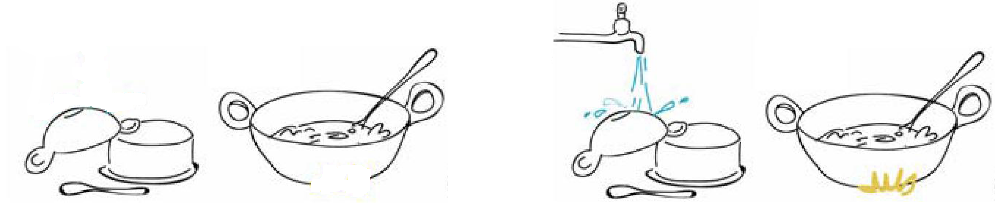
\includegraphics[width=1.00\textwidth]{Daten/pic_fail2.PNG}
	\caption{Deutlichkeit der Illustrationen $^{\ref{MedhiSagarKentaro01}}$}
	\label{fig:picfail}
\end{figure}

Die erste Anwendung soll dem Benutzer eine Karte anzeigen, die ihm helfen soll, seinen Zielort zu erreichen, wie in Abbildung \ref{fig:mapsimple}.\\
"Ubliche Karten arbeiten mit Stra"sennamen, welche einen Analphabeten jedoch nicht weiterhelfen. Somit soll der Benutzer sich  hier an Merkmalen der Stra"sen wie Gesch"aften, Krankenh"ausern, oder Bushaltestellen zurechtfinden.
Bei der ersten Version dieser Anwendung wurde die Person als Pfeil und die zu gehenden Wege in Blau markiert. Jedoch f"uhrte das zu Missverst"andnissen mit den Probanden. So wurde der Weg als Fluss gedeutet und der Pfeil erst gar nicht wahrgenommen. Darum ersetzten die Entwickler die Stra"sen mit Grau und den markierten die Wegbeschreibung durch einen dunkleren Grauton und einer dickeren Linie.
Auch der Pfeil wurde durch eine Figur ersetzt, welche je nach Richtung entweder von vorne, hinten oder der Seite zu sehen ist.

\begin{figure}[h]
	\centering
		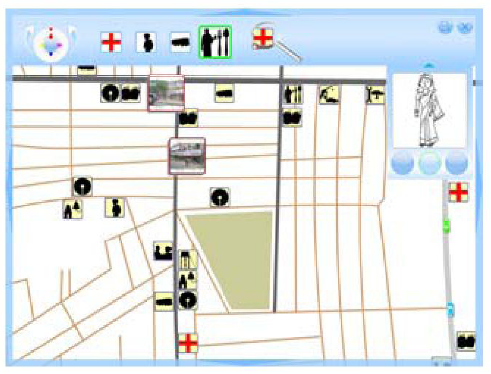
\includegraphics[width=0.8\textwidth]{Daten/map_simple.PNG}
	\caption{Vereinfachte Karte $^{\ref{MedhiSagarKentaro01}}$}
	\label{fig:mapsimple}
\end{figure}
Die zweite Anwendung soll dem Benutzer eine Art Job-B"orse bieten und somit einen besseren Anschluss an die restliche Bev"olkerung bieten.\\
Dabei wird ebenfalls vollst"andig auf geschriebenen Text verzichtet, sodass Analphabeten leicht mit der Anwendung umgehen k"onnen.
Was allerdings nicht auf den folgenden Abbildungen zu sehen ist, ist die Sprachausgabe die "uber die Hilfe zu jeder Information m"oglich ist. Klickt der Benutzer auf die Hilfe wird zur jeweiligen Ansicht die n"otigen Informationen und Verwendungsm"oglichkeiten erz"ahlt.
In der Abbildung \ref{fig:joblist} ist zu erkennen wie die Anwendung nur aus Bildern besteht. Die Abbildung zeigt eine Liste von Jobs. Wie der Benutzer zu dieser Auswahl gelangt oder wodurch sie bestimmt wird, wurde nicht erw"ahnt.\\
\begin{figure}[h]
	\centering
		\includegraphics[width=0.80\textwidth]{Daten/job_list.PNG}
	\caption{Job Liste basierend auf Bildern $^{\ref{MedhiSagarKentaro01}}$}
	\label{fig:joblist}
\end{figure}
Das stadt"ahnliche Symbol links soll zeigen, ob der Arbeitsplatz in der Stadt liegt oder nicht. In der Mitte sind die geforderten Aufgaben zu erkennen. Danach wird die f"ur den Ort "ubliche Uhr als Zeitangabe mit Mond und Sonne als Zeichen f"ur Vor- und Nachmittags dargestellt. Da in der Studie beobachtet wurde, dass die Probanden keine Probleme mit Zahlen hatten, wird ganz rechts der Lohn als Geldschein mit dem Wert gezeigt.\\
Die Hilfe ist "uber das Portrait zu finden, da es den meisten Probanden leicht fiel ein Portrait einer beliebigen Person als Hilfe wahrzunehmen. Um nun eine detailliertere Ansicht des Berufs zu erhalten, muss der Proband nur auf die passende Reihe klicken und kommt so zur Abbildung \ref{fig:jobclose}.
Hier sind die Informationen noch einmal genauer aufgef"uhrt. Oben in der Mitte wird die Arbeitszeit nun auch mit Ende, bzw. mit Unterbrechung angegeben. Der Lohn steht nun auch in Geldscheinen in der rechten Ecke. Auch steht nun bei jeder T"atigkeit dabei, welchem Lohn sie entspricht, damit der Bewerber den Aufwand erkennen kann. Zum Schluss finden sich unten die Angaben, in welchen und wie vielen R"aume etwas zu tun ist.

\begin{figure}[h]
	\centering
		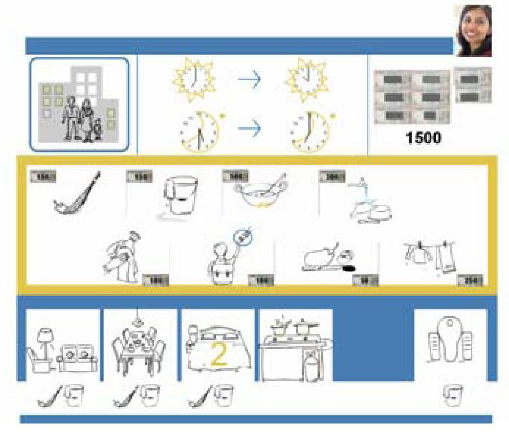
\includegraphics[width=0.7\textwidth]{Daten/job_close.PNG}
	\caption{Job Ansicht $^{\ref{MedhiSagarKentaro01}}$}
	\label{fig:jobclose}
\end{figure}

\clearpage


	\section{Anwendungen}
	\subsection{Invisque (Interactive VIsual Search and Query Environment)}
		
\frame{\frametitle{Was ist Invisque?}
	\begin{itemize}
		\item Prototyp zur interaktiven und anschaulichen Suche
		\item Basierend auf Schreibtisch und Karteikarten Metapher
		\item Für \glqq Leseschwache\grqq in Industrienation 
	\end{itemize}
}

\frame{\frametitle{Design Gedanken}
	%dem benutzer weniger gedanken an die bedienung verschwenden lassen
	\begin{itemize}
		\item kleine Informationsstücke
		\item aufgeräumte Darstellung (\glqq page clutter\grqq)
		\item Freiraum und Farbe
		\item Animationen
		\item Verschachtelung verringern
	\end{itemize}
}

\frame{\frametitle{Evaluation}
\begin{columns}
	\column{0.5\textwidth}
	\begin{itemize}
		\item 24 Testpersonen
		\item zwölf Frauen und zwölf Männer
		\item zwölf \glqq Lesestarcke\grqq und zwölf \glqq Leseschwache\grqq
		\item zwischen 35 und 50 Jahre alt
		\item zwischen fünf und zehn Stunden Computer- und Internetnutzung in der Woche
		%bild der Ergebnisse
	\end{itemize}
	%\column{0.5\textwidth}
\end{columns}
}

\frame{\frametitle{Demo}

}

	\subsection{Jobb"orse}
		\frame{\frametitle{Job-B"orse}%Ziel: entwicklung von Anwendungen zur freien und unabhängigen benutzung durch Analphabeten
	\begin{center}
		"Text-freie Benutzereingabe für Analphabeten und semi-gebildete Benutzer"\\
		\vspace*{0.5cm}
		Indrani Medhi, Aman Sagar und Kentaro Toyama\\
	\end{center}
	2006
}
\frame{\frametitle{Testpersonen}
	60 Personen aus 3 Urban-Slums in Indien:\\
	\begin{itemize}
		\item Muttersprache meist Kannada
		\item meist Analphabeten
		\item keine Erfahrung mit Computer
		\item Berufsspanne:
		\begin{itemize}
			\item Haushälter/in
			\item Hausmeister
			\item Bauarbeiter
			\item ...
		\end{itemize}
	\end{itemize}
}

\frame{\frametitle{Designschlüsse}
	\begin{itemize}
		\item vermeiden von Text
		\item Nummern sind verständlich
		\item Audioausgabe
		\item Hilfe anbieten
		\item Bilder verwenden
		\item Kultur berücksichtigen 
		\item höherer Detailgrad bei Zeichnungen
	\end{itemize}
}
\frame{\frametitle{Kultur}
	\begin{figure}
		\centering
		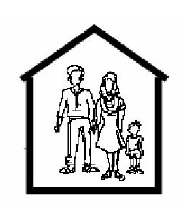
\includegraphics[width=\textheight]{Slides/Anwendungen/Daten/pics/town.PNG}
	\end{figure}\pause
	\begin{figure}
		\centering
		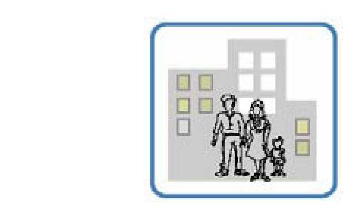
\includegraphics[width=\textheight]{Slides/Anwendungen/Daten/pics/town2.PNG}
	\end{figure}
}
\frame{\frametitle{Detailgrad}
	\begin{figure}
		\centering
		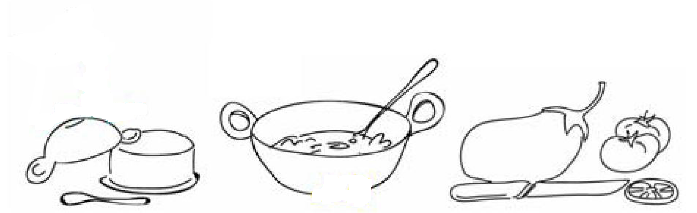
\includegraphics[width=\textheight]{Slides/Anwendungen/Daten/pics/detail_ohne.PNG}
	\end{figure}
}
\frame{\frametitle{Detailgrad}
	\begin{figure}
		\centering
		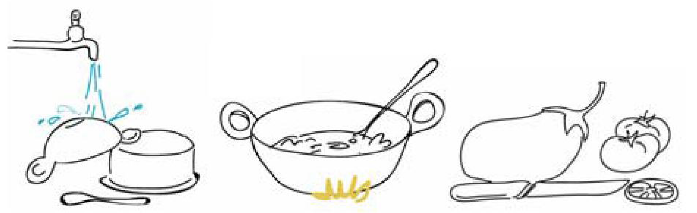
\includegraphics[width=\textheight]{Slides/Anwendungen/Daten/pics/detail_mit.PNG}
	\end{figure}
}
	\frame{\frametitle{Prototyp-Map}
		\begin{figure}
			\centering
			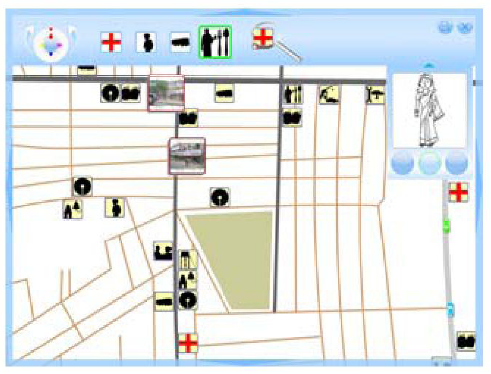
\includegraphics[width=\textheight]{Slides/Anwendungen/Daten/pics/map.PNG}
		\end{figure}
	}
	\frame{\frametitle{Prototyp-Auswahl}
		\begin{figure}
			\centering
			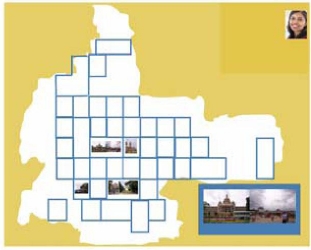
\includegraphics[width=\textheight]{Slides/Anwendungen/Daten/pics/job_map.PNG}
		\end{figure}
	}
	\frame{\frametitle{Prototyp-Auswahl}
		\begin{figure}
			\centering
			\includegraphics[width=\textheight]{Slides/Anwendungen/Daten/pics/job_list.PNG}
		\end{figure}
	}
	\frame{\frametitle{Prototyp-Job}
		\begin{figure}
			\centering
			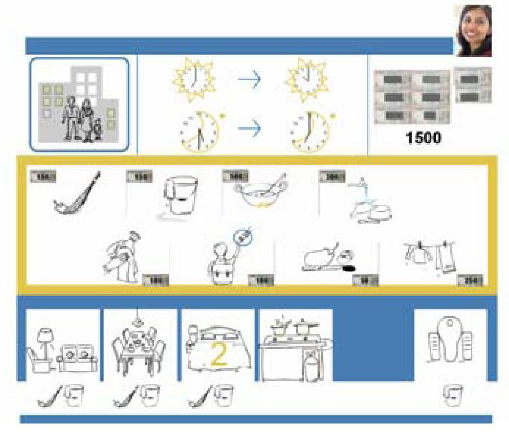
\includegraphics[width=\textheight]{Slides/Anwendungen/Daten/pics/job.PNG}
		\end{figure}
	}

	\frame{\frametitle{Test}
		 Getestet wurden:\\
		\begin{itemize}
			\item Prototyp mit Hilfe
			\item Prototyp ohne Hilfe
			\item Herkömmliche Anwendung mit identischen Inhalt
		\end{itemize}\pause
	\vspace*{0.5cm}
		\begin{itemize}
			\item Ist die herkömmliche Anwendung zug"anglich für die Testgruppe?
			\item Sind die Designschlüsse ausreichend für die Testgruppe?
			\item Welche Anwendung ist am zug"angiger?
		\end{itemize}
	}
	% herkömmliche Anwendung ist nicht anwendbar
	% funktionsweise schnell erkannt, inhalt unschlüssig
	% voice feedback ist "funny" und hilfreich
	% benutzer gruppen kahmen besser zurecht
	% hilfe beruhigt und bechleunigt anwendung
	% navigation wie ein buch zugänglicher
	\subsection{DVV-Lernportal}
		\frame{\frametitle{DVV-Lernportal}
			Deutscher Volkshochschul-Verband e. V. \\
			Lernportal ich-will-lernen.de \\
			\begin{figure}
				\centering
				
\includegraphics[width=\textheight]{Slides/Anwendungen/Daten/pics/ich-will-lernen.jpg}
			\end{figure}
		}

\section*{}
 \frame{\frametitle{}
 	\begin{center}
    		\huge Ende\\
    			Vielen Dank
	\end{center}
 	
 }
	
%Zahl der Betroffenen
	%weltweit
	%deutschland
	%vergleich zu anderen behinderungen

%Pers"onliche auswirkungen

%Was ist Analphabetismus?
	%analphabeten sind nicht dumm!
	%abstufungen von Analphabetismus
	%ursachen von analphabetismus

%Teilgruppen der Analphabeten
	%Legasteniker
	%lern schwache, lern behinderte
	%funktionale Analphabeten

%Demonstration wie sich analphabetismus anf"uhlt
	%Text oder Programm in fremder Sprache
		%Merkaartor in Niederl"andisch?

%Beeintr"achtigungen
	%lesen
	%errinerungsvermögen
	%"Denken "ubers Denken"
	%Orientierung (in dokumenten) und suche

%Design l"osungen
	%alphabetisierung.de
		%readspeaker.com
	%interactive visualization for low literacy users
		%nicht f"ur legastheniker
	%Textvermeidung
		% Zahlen werden von den meisten jedoch dennoch richtig identifiziert.

%Design testen
	%probanden finden
	%zusammenarbeit mit Probanden


\end{document}
